\documentclass[12pt]{scrartcl}
\usepackage{config}
\usepackage{minted}
\usepackage[utf8]{inputenc}
%\newcommand\mrh{\color{white}\bfseries}
\newcommand\mrc[1]{\begin{tabular}{@{}l@{}} #1 \end{tabular}}
\setlength\arrayrulewidth{0.8pt}

\usemintedstyle{pastie}

\begin{document}
    \hh{Niccori\^{}\^{}  Survey Team}

    \vspace{10pt}

    \hh{Problem}

        In their odyssey to survey all the smiles in the world, Rin and Ren have arrived in Ecatepec. Ecatepec can be seen as a graph with $N$ vertices, numbered from $0$ to $N - 1$, connected by some bidirectional edges. However, since it is largely uncharted territory, the team does not know about its edges. If Ecatepec turns out to be disconnected\footnote{We say that a graph is connected if for every pair of vertices, there is a path (a sequence of vertices such that each pair of adjacent vertices is connected by an edge) that starts at one and ends at the other.}, Rin and Ren will not be able to carry out their mission properly, so they enlist the help of the great scientist Miku. Miku gives our adventurers a curious device that answers questions as follows given a parameter $K$ that Miku has set beforehand:

        Given two distinct vertices of the Ecatepec graph, the device answers whether they are at a distance\footnote{The distance between two vertices is defined as the path with the fewest edges connecting them, expressed as $dist(a, b)$.} less than $K$, exactly $K$, or greater than $K$.

        Since the device is still a prototype, Miku warns the team that they can ask at most $\frac{2N^2}{K}$ questions. Rin and Ren failed math in high school, so they enlist your help to determine if Ecatepec is connected.
        

    \hh{Implementation Details}

        You must implement the function \textit{Equipo\_sonrisas()}. This function receives an integer $N$ (the size of the graph) and an integer $K$ (the device's parameter). This function should return a pair of integers: if the graph is connected, it should return the pair $(-1, -1)$. If the graph is not connected, it should return a pair of vertices in different components. 
        
        During your program, you can call the function \textit{Dispositivo\_Miku()}. This function receives 2 integers $a, b$ and returns $-1$ if $dist(a, b) < K$, $0$ if $dist(a, b) = K$, and $1$ if $dist(a, b) > K$.
        To call this function, you must include the library \textit{``Sonrisas.h"} with the command \textit{\#include ``Sonrisas.h"}.
        An example program would look like this:

\begin{minted}{c++}
#include "Sonrisas.h"
#include <bits/stdc++.h>
using namespace std;

pair<int, int> Equipo_sonrisas(int N, int K) {
    // Implement this function.
}

\end{minted}

    The grader will call this function \textbf{multiple} times for each testcase.
    
    \hh{Example}

        \begin{itemize}
            \item The grader calls the function 
            \begin{center}
                \textit{Equipo\_sonrisas(5, 2)}
            \end{center}
            The hidden graph is as follows:
            \begin{center}
                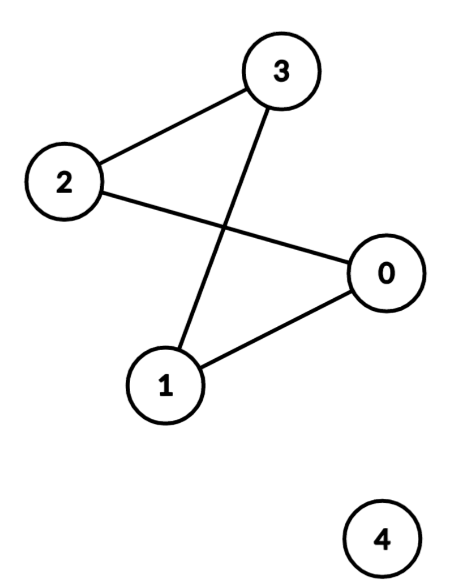
\includegraphics[scale=0.3]{ej1.png}
            \end{center}
            \item the following is a distance table of the graph:
            
            \begin{center}
                \begin{tabular}{|c||c|c|c|c|c|}
                    \hline
                    $dist(a, b)$ & 0 & 1 & 2 & 3 & 4 \\
                    \hline
                    \hline
                     0 & 0 & 1 & 1 & 2 & $\infty$ \\
                     \hline
                     1 & 1 & 0 & 2 & 1 & $\infty$ \\
                     \hline
                     2 & 1 & 2 & 0 & 1 & $\infty$ \\
                     \hline
                     3 & 2 & 1 & 1 & 0 & $\infty$ \\
                     \hline
                     4 & $\infty$ & $\infty$ & $\infty$ & $\infty$ & 0 \\
                     \hline 
                \end{tabular}
            \end{center}
            \item Here is an example interaction:
            \begin{center}
                \begin{tabular}{|c|c|}
                    \hline
                     Function called &  return value \\
                     \hline 
                     \hline 
                     \textit{Dispositivo\_Miku(0, 1)} & -1 \\
                     \hline 
                     \textit{Dispositivo\_Miku(0, 2)} & -1 \\
                     \hline 
                     \textit{Dispositivo\_Miku(0, 3)} & 0 \\
                     \hline 
                     \textit{Dispositivo\_Miku(0, 4)} & 1 \\
                     \hline 
                     \textit{Dispositivo\_Miku(1, 2)} & 0 \\
                     \hline 
                     \textit{Dispositivo\_Miku(1, 3)} & -1 \\
                     \hline 
                     \textit{Dispositivo\_Miku(1, 4)} & 1 \\
                     \hline 
                     \textit{Dispositivo\_Miku(2, 3)} & -1 \\
                     \hline 
                     \textit{Dispositivo\_Miku(2, 4)} & 1 \\
                     \hline 
                     \textit{Dispositivo\_Miku(3, 4)} & 1 \\
                     \hline 
                \end{tabular}
            \end{center}
            \item If the return value of the function called by the grader is $(-1, -1)$, the veredict would be wrong answer. Otherwise, if the return value is, for example, $(1, 4)$, the veredict would be accepted.
        \end{itemize}
        
    \hh{Constraints}
        \begin{itemize}
            \item $1 \le K < N \le 1000$.
            \item In all cases, the number of times you call the function \textit{Dispositivo\_Miku()} must be less than $\frac{2N^2}{K}$. Otherwise, you will receive a wrong answer veredict.
            \item If the function returns $(-1, -1)$ and the graph is not connected, or if it returns a pair of connected nodes, you will receive a wrong answer veredict.
            \item Let $S_N$ be the sum of the values of $N$ for each call made by the grader in a testcase. It is guaranteed that $S_N \le 1000$.
        \end{itemize}
    
    \hh{Subtasks}

    \begin{itemize}
        \item (5 points) $K = N - 1$.
        \item (10 points) $K \le 4$.
        \item (33 points) $K = \frac{N}{2}$.
        \item (22 points) The graph is a forest (there are no cycles, that is, there is no paths that don't repeat edges and start and end at the same vertex).
        \item (30 points) No additional constraints.
    \end{itemize}
\end{document}
